\documentclass[
BCOR0.7cm,							% Bindekorrektur, bspw. 1 cm
]
{scrbook}

\newif\ifpdf
\ifx\pdfoutput\undefined
	\pdffalse              	%normales LaTeX wird ausgef�hrt
\else
	\pdfoutput=1           
	\pdftrue               	%pdfLaTeX wird ausgef�hrt
\fi

\ifpdf
	%\usepackage{ae}        % Benutzen Sie nur
	%\usepackage{zefonts}  	% eines dieser Pakete
\else
	%%Normales LaTeX - keine speziellen Fontpackages notwendig
\fi

\ifpdf %%Einbindung von Grafiken mittels \includegraphics{datei}
	\usepackage[pdftex]{graphicx} %%Grafiken in pdfLaTeX
\else
	\usepackage[dvips]{graphicx} %%Grafiken und normales LaTeX
\fi


\ifpdf
	\pdfinfo
	{
    /Author (Christian Paminger)                                
    /Title (FAS-Online)     
    /Subject (Benutzerhandbuch FAS-Online)                                    
    /Keywords (FAS FH-Complete Technikum-Wien)
	}
\else			
\fi

\usepackage{listings} \lstset{numbers=left, numberstyle=\tiny, numbersep=5pt}
\lstset{language=tex} 
\usepackage{color}
\definecolor{linkfarbe}{rgb}{0.5,0.5,0.5}
\usepackage[pdftex,colorlinks=true,urlcolor=linkfarbe,linkcolor=linkfarbe]{hyperref}
\usepackage[ngerman]{babel}		
\usepackage[T1]{fontenc}
\usepackage[latin9]{inputenc}
\usepackage{makeidx}
\usepackage{float}
\usepackage[small,bf]{caption}
\usepackage{fancyhdr}
\usepackage{amssymb,amsmath}
\makeindex

\graphicspath{{../../images/}}

\setlength{\parindent}{0pt}
\setlength{\parskip}{1ex plus 0.5ex minus 0.2ex}
\addtolength{\textheight}{2cm}
\addtolength{\headheight}{2pt}
\setlength{\captionmargin}{20pt}
\floatstyle{plain}
\floatname{example}{Example}

\newfloat{example}{hbtp}{loe}[chapter]
\floatplacement{figure}{hbtp}
\floatplacement{table}{htbp}

\newcommand{\dollar}{\char36}

\newenvironment{info}[1]{
    \hspace{-10mm}
    \fbox{
        \begin{minipage}{1cm}
        
\includegraphics[width=1cm]{icon_info}
        \end{minipage}
        \begin{minipage}{14.5cm}
        #1
        \end{minipage}
    }
}

\newenvironment{achtung}[1]{
    \hspace{-10mm}
    \fbox{
        \begin{minipage}{1cm}
        
\includegraphics[width=1cm]{icon_achtung}
        \end{minipage}
        \begin{minipage}{14.5cm}
        #1
        \end{minipage}
    }
}

\newenvironment{halt}[1]{
    \hspace{-10mm}
    \fbox{
        \begin{minipage}{1cm}
        
\includegraphics[width=1cm]{icon_halt}
        \end{minipage}
        \begin{minipage}{14.5cm}
        #1
        \end{minipage}
    }
}

\newenvironment{idee}[1]{
    \hspace{-10mm}
    \fbox{
        \begin{minipage}{1cm}
        
\includegraphics[width=1cm]{icon_idee}
        \end{minipage}
        \begin{minipage}{14.5cm}
        #1
        \end{minipage}
    }
}


\setlength{\unitlength}{1mm}

\newenvironment{markier}[5]{
    
    \thicklines \put(#2,#3){\vector(#4,#5){5}} \thinlines
    \put(#2,#3){\circle*{5}}
    \put(#2,#3){\textcolor{black}{\circle{5}}\makebox(-10,0){\textcolor{white}{#1}}}


}


\hyphenation{gleich-zeitig para-meter}


\begin{document}

\ifpdf
	\DeclareGraphicsExtensions{.pdf,.jpg,.png}
\else
	\DeclareGraphicsExtensions{.eps}
\fi

\pagestyle{fancyplain}
% Titelseite einbinden
%%
% Titelseite, Abstrakt, Danksagung und Inhaltsverzeichnis
%
%% eigene Titelseitengestaltung %%%%%%%%%%%%%%%%%%%%%%%%%%%%%%%%%%%%%%%    

\begin{titlepage}
\begin{center}
\vspace*{40mm} \huge Benutzerhandbuch\\
\vspace*{10mm}
\vfill 
\includegraphics[width=130mm]{logo_fas}
	
\large \vfill \textsc{Technikum Wien}\\

Wien, \today
\end{center}
\end{titlepage}


\tableofcontents			% Inhaltsverzeichnis
%\listoftables				% Tabellenverzeichnis
\listoffigures				% Abbildungsverzeichnis

\frontmatter					% Vorspann (z.B. r�mische Seitenzahlen)

\chapter{Vorwort}


\mainmatter						% Hauptteil

%% Kapitel Anfang %%%%%%%%%%%%%%%%%%%%%%%%%%%%%%%%%%%%%%%%%%%%%%%%%



\setchapterpreamble[u]{%
\dictum[\LaTeX, 1. Gebot]{Thou shallst concentrate on the content}}
\chapter{\LaTeX~f�r TW-Dokumentation}


\newpage
\section{Allgemeines}
\subsection{\LaTeX}

Aus der \LaTeX-Doku:
\begin{quote}
LaTeX is a document preparation system for high-quality typesetting. It is
most often used for medium-to-large technical or scientific documents but it
can be used for almost any form of publishing.

LaTeX is not a word processor! Instead, LaTeX encourages authors not to worry
too much about the appearance of their documents but to concentrate on getting
the right content.
\end{quote}

Online Befehlsreferenz: http://www.weinelt.de/latex/index.html

\subsection{Einbindung der Vorlage}

\begin{enumerate}
\item svn: template.tex aus dem TeX-Verzeichnis ins eigene Handbuchverzeichnis
kopieren (e.g. FAS)
\item alte Zentraldatei (FASo.tex) umbenennen in FASo\_old.tex
\item Kopie von template.tex umbenennen in FASo.tex
\item Kapitel-includes aus FASo\_old.tex in FASo.tex kopieren
\end{enumerate}

\section{Bilder}
\subsection{Format}

\begin{itemize}
\item Screenshots im PNG-Format speichern
\item Benamsung: dokumentname\_kapitelname\_bildname.png\\
(e.g. CIS\_benotungstool\_notenschluessel.png)
\item Im Bildbearbeitungsprogramm Ausgabebreite auf 140mm stellen ->
errechnete H�he f�r picture - Umgebung wichtig
\end{itemize}

\newpage
\subsection{Einbindung}

\begin{figure}[htbp]
    \begin{center}
        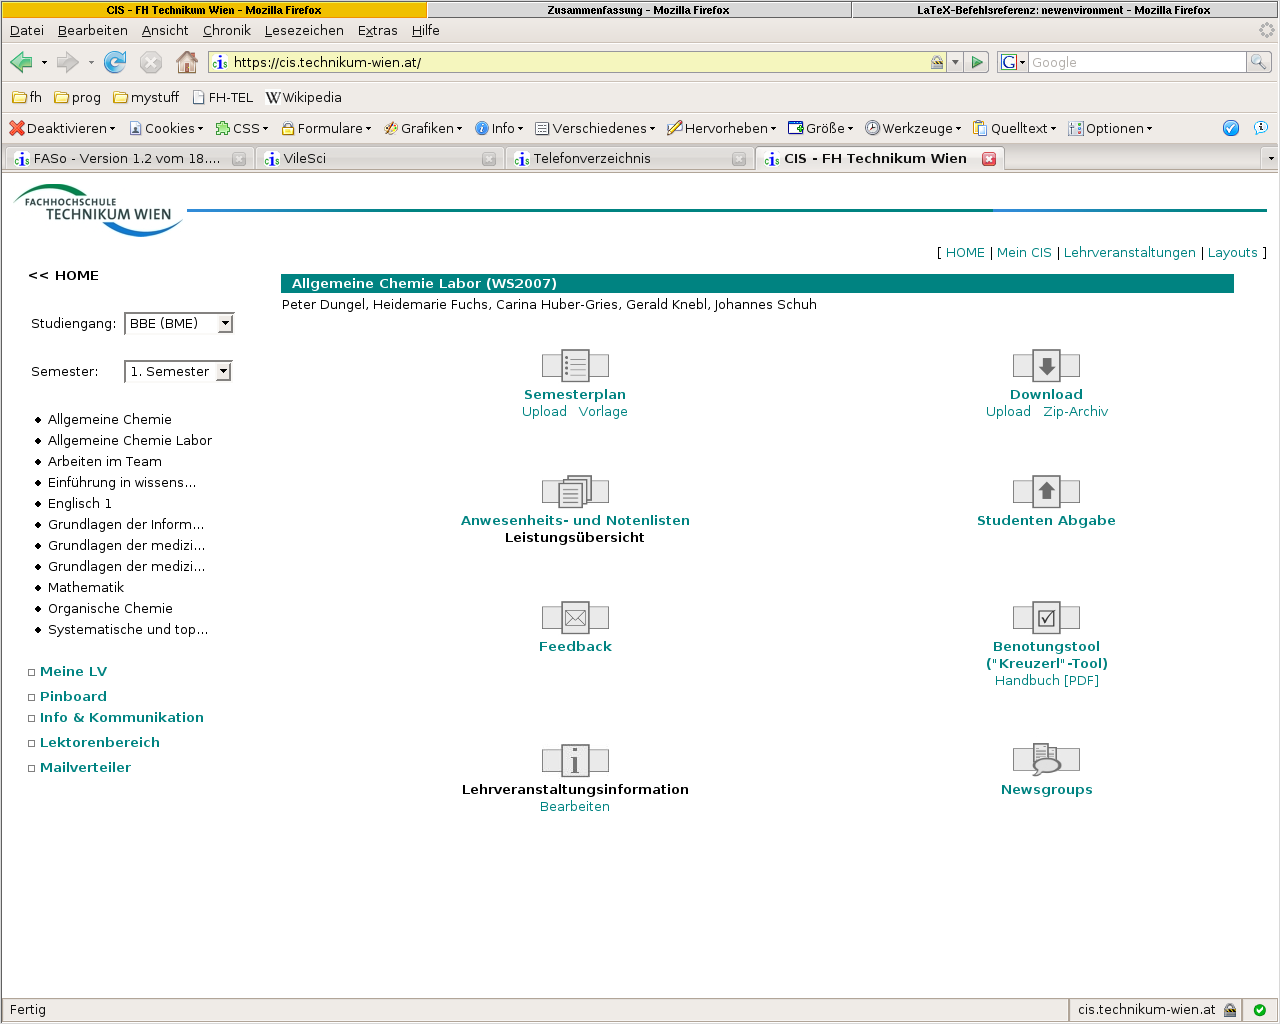
\includegraphics[width=0.9\textwidth]{dummy}
        \caption{Einfache Einbindung eines Bildes ohne Marker}
        \label{foo}
    \end{center}
\end{figure}

\begin{lstlisting}[caption=Code zu Abb. \ref{foo}]
\begin{figure}[htbp]
    \begin{center}
        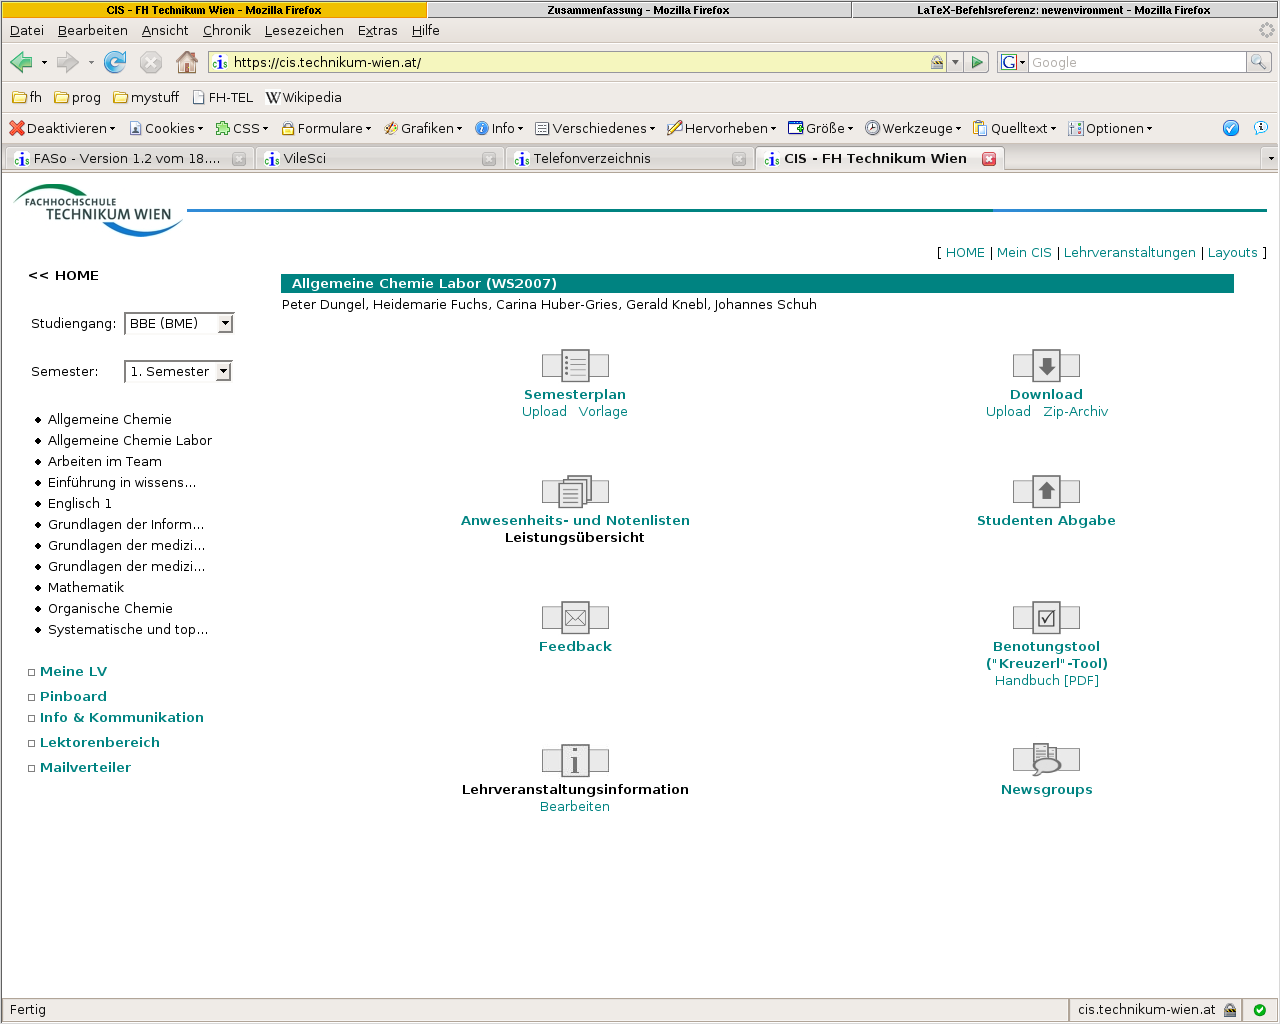
\includegraphics[width=0.9\textwidth]{dummy}
        \caption{Einfache Einbindung eines Bildes ohne Marker}
        \label{foo}
    \end{center}
\end{figure}
\end{lstlisting}


\newpage

\begin{figure}[htbp]
    \begin{center}
        \begin{picture}(140,112)
            \put(0,0){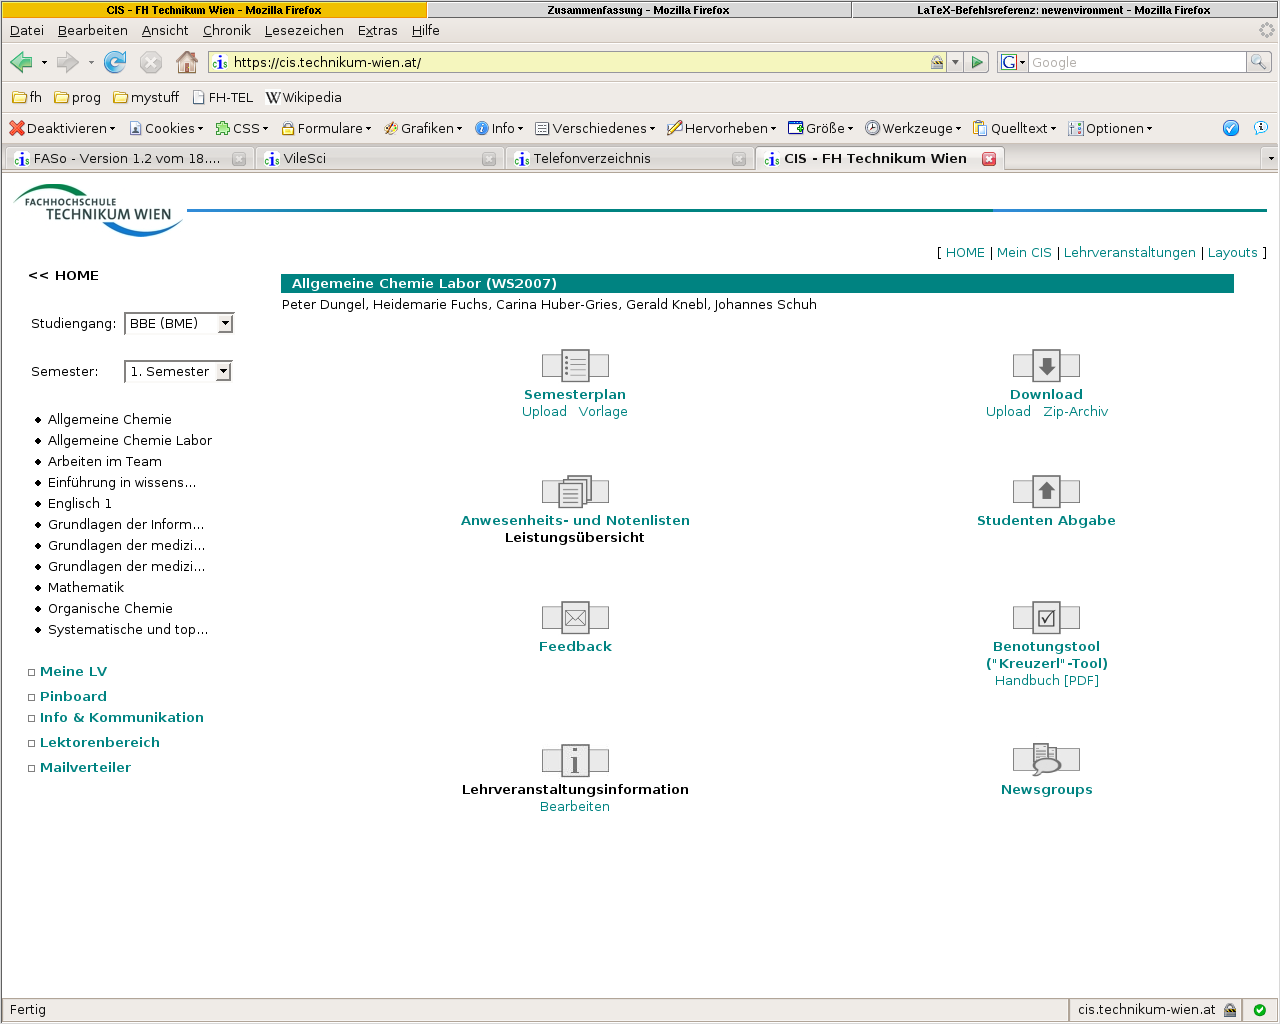
\includegraphics[width=140mm]{dummy}}
            \markier{1}{50}{36}{1}{1}
            \markier{2}{105}{36}{1}{-1}

        \end{picture}
        \caption{Einbindung eines Bildes mit 2 Markern}
        \label{bar}
    \end{center}
\end{figure}

\begin{lstlisting}[caption=Code zu Abb. \ref{bar}]
\begin{figure}[htbp]
    \begin{center}
        \begin{picture}(140,112)
            \put(0,0){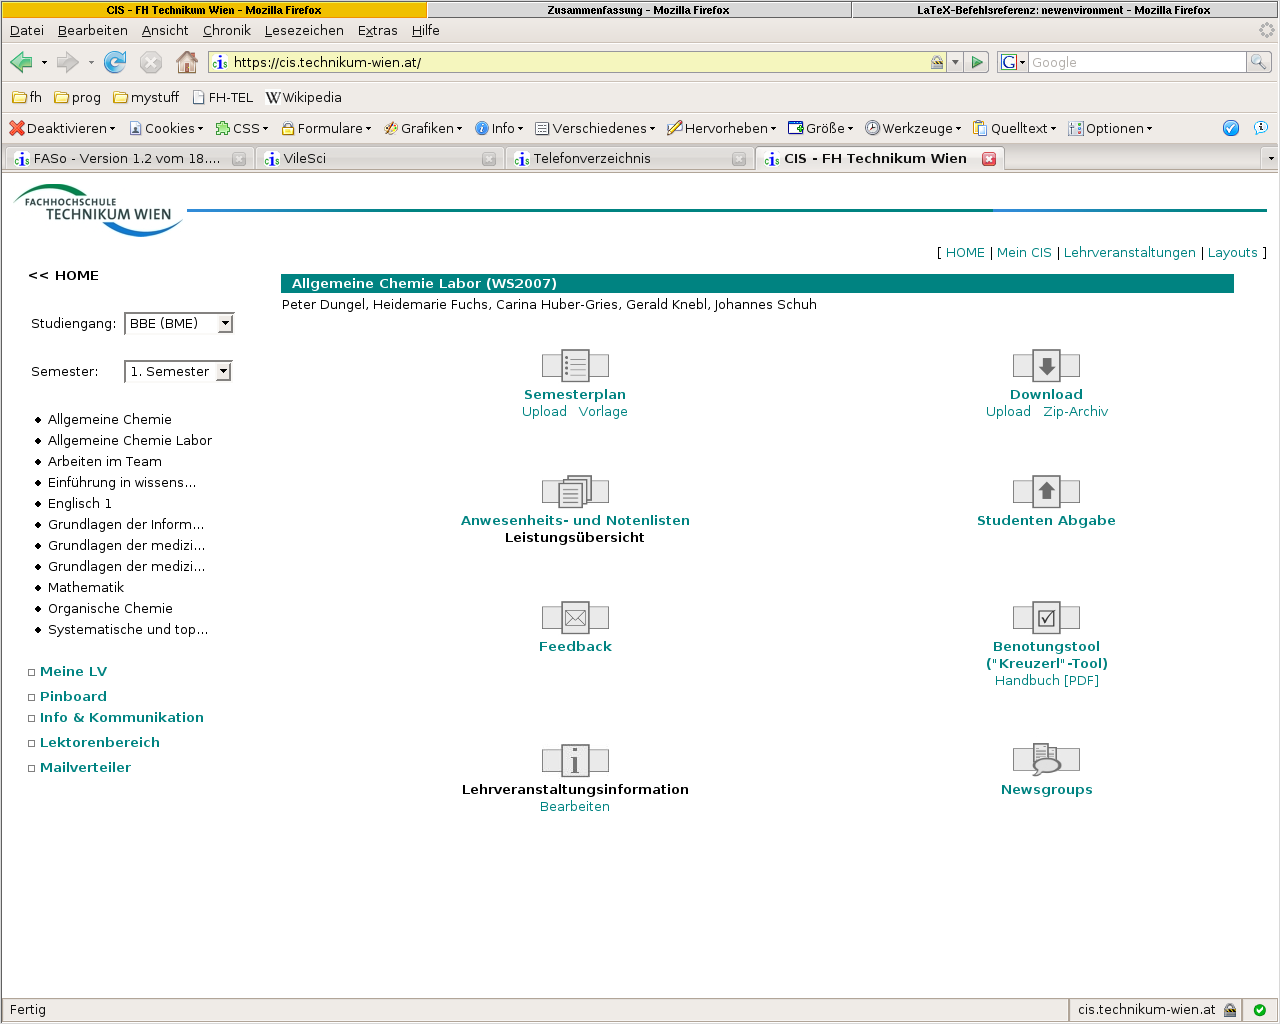
\includegraphics[width=140mm]{dummy}}
            \markier{1}{50}{36}{1}{1}
            \markier{2}{105}{36}{1}{-1}
        \end{picture}
        \caption{Einbindung eines Bildes mit 2 Markern}
        \label{bar}
    \end{center}
\end{figure}
\end{lstlisting}

Details zur markier-Umgebung:
\begin{lstlisting}
\markier{nummer}{x}{y}{vector_x}{vector_y}
\end{lstlisting}

\textbf{nummer}: dargestellte Zahl, \textbf{x, y}: Kreiszentrum von links
unten in mm, \textbf{vector\_x, vector\_y}: Steigung des Pfeiles: Zahlen von -4 bis +4

\achtung{Die H�he der picture-Umgebung muss dem Screenshot angepasst
werden!\\ Angabe in mm; hier: (140,\textbf{112})}

\subsection{Referenzierung}


\ldots\\
Feedback an den LV-Leiter k�nnen Sie �ber den Link \textit{Feedback} (s. Abb.
\ref{bar} Pkt. 1 auf S. \pageref{bar}) senden. \\
\ldots\\

\begin{lstlisting}[]
(s. Abb. \ref{bar} Pkt. 1 auf S. \pageref{bar})
\end{lstlisting}


\section{Boxen}

\achtung{Achtung!}

\idee{Idee, Tipp}

\halt{\textbf{HALT!}}

\info
{
    \begin{tabular}[t]{p{40mm}|cp{70mm}}
        \cline{1-3}
        9. Oktober 2007&-& Infomail der freigegebenen Noten beinhaltet nun auch die
        Note\\
        \cline{1-3}
    \end{tabular}
}

\begin{lstlisting}[]


\achtung{Achtung!}

\idee{Idee, Tipp}

\halt{\textbf{HALT!}}

\info
{
    \begin{tabular}[t]{p{40mm}|cp{70mm}}
        \cline{1-3}
        9. Oktober 2007&-& Infomail der freigegebenen Noten 
        beinhaltet nun auch die Note\\
        \cline{1-3}
    \end{tabular}
}

\end{lstlisting}



%% Kapitel Ende   %%%%%%%%%%%%%%%%%%%%%%%%%%%%%%%%%%%%%%%%%%%%%%%%%


\appendix							% Beginn des Anhangs
\chapter{Schluss}


\end{document}
